% \begin{figure}
%     \caption{Hypothesis Model}
%     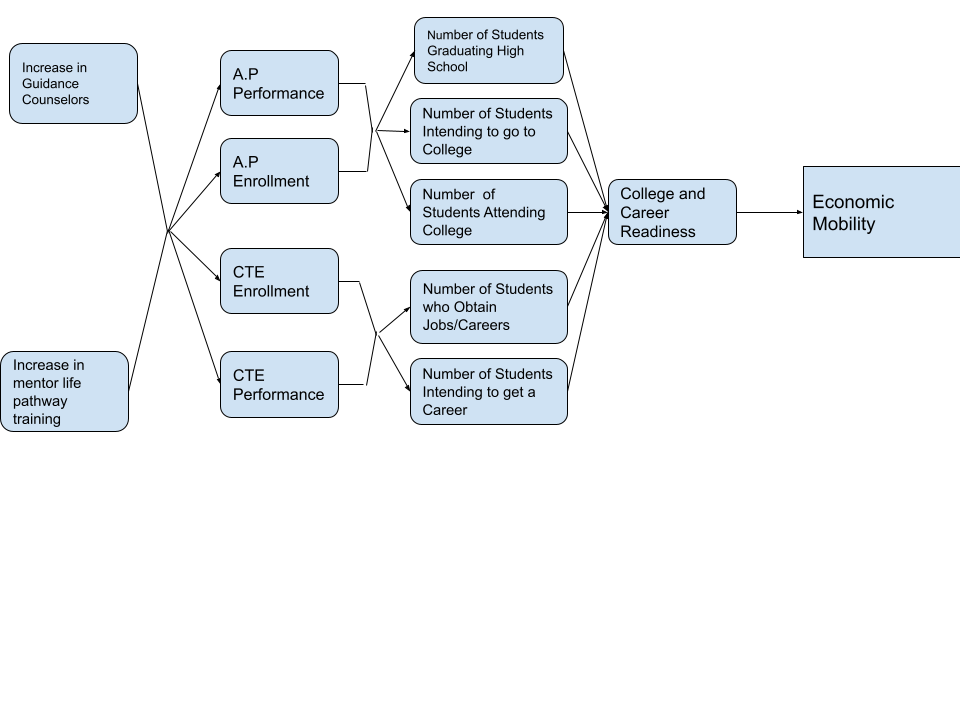
\includegraphics[width=16cm]{updated_hypothesis_model.png}
%     \label{fig3}
% \end{figure}

\textbf{Hypothesis 1} \textit{As the number and life pathway training of mentors increase, their instruction will lead to an increase in high school academic performance, leading to higher college enrollment rates for low-socioeconomic students.}

A postsecondary education has been the traditional path towards a well-paying career and remains the primary goal of many high school students with plans after high school. 
Low income students have been shown to have attitudes opposing college or not have the usual educational experiences that are consistent with four-year degree students \parencite[][]{king1996}. 
The cost associated with a university education can often dissuade low income students from wanting to attend \parencite[][]{king1996}
Stereotype threat can be detrimental to a student's self-worth and potential \parencite[][]{croizet1998}.
A student that does not see themselves in successful positions will not take the steps necessary to achieve those goals. 
These perceptions need to be changed through active intervention from our schools and mentors that interact with students. 
Proactive intervention by counselors has been shown to have a positive effect on students' attitudes towards school  and testing performance \parencite[][]{lee1993}.
Guidance counselors are a boon in the confusing college application environment. 
Their knowledge of the process, schools, and costs associated with enrolling in postsecondary education is essential to students, especially those of low-socioeconomic status, who often do not fully understand the financial burdens associated with college \parencite[][]{castleman2014intensive,deslonde2018high}. 
The duties for a counselor can go beyond just the choice and application of schools \parencite[][]{deslonde2018high}.  
In schools with majority Black students and numerous students eligible for reduced lunches, the role of counselors extends beyond that of college applications, to mentorship in all areas of life where the student may face barriers \parencite[][]{farmer2006}.
With the racial and income segregation apparent in CMS schools, more effective and socially equipped counselors are a necessity to achieve educational equity. 
Access to a counselor provides students with the social capital available to the counselor \parencite{tang2019high}. 
Counselors may have contacts, knowledge of helpful resources, and beneficial programs to supplement students' efforts in succeeding academically, both in secondary school and postsecondary. 

The variables to operationalize the concepts in hypothesis 1 is the ratio of guidance counselors to students throughout CMS high schools. 
High school graduate intentions will be used to determine the training of counselors, a lagging indicator of bias and discrimination training. 
Academic performance is AP participation rate in each school, and the passing rate for AP exams. 
A three or more is considered passing for this variable. College enrollment rates will be for economically disadvantaged students in each school. 
Further hypothesis 1 development and additional variables will be discussed later in this paper.


\textbf{Hypothesis 2} \textit{As the quality and number of mentors increase, there will be an increase in obtained CTE Credentials by students within Charlotte Mecklenburg County Schools.}

The catalyst for economic mobility is not only related to postsecondary attainment, but technical and middle-skill jobs provide opportunities for growth and upward mobility \parencite[][p. 27]{LOO}
Research results suggest that proactive engagement with students often has a direct impact on academic performance, career selection, and postsecondary decisions \parencite[][]{lee1993}. 
An example of this is Magnuson and Starr's paper, `How early is too early to begin life career planning? the importance of the elementary school years', it was shown that academic guidance and life pathway instruction beginning at an early age are more likely to rise in economic status (\citedate{magnuson2000}). 
This deliberation and perspective on their future allowed for a more successful transition into secondary students and beyond into prosperous careers, including technical employment.
This early consideration leads to a well-informed decision in career selection, giving students that may prefer a technical vocation to that of a postsecondary degree. 
Early childhood habits help familiarize students with their occupational preferences, competence, and parameters of success in their chosen field \parencite[][]{magnuson2000}.

\blockquote[(unpublished work) Kadka et al., 2021]{
    The literature suggests that parents, educators, and counselors should emphasize the pursuit of vocations within the United States, primarily because of its dichotomy of historical attrition and increased necessity; 
    this ideal was additionally supported by the Perkins Career and Technical Education (CTE) Act of 2006 \parencite{castellano2017}}

The variables to be operationalized in order to test hypothesis 2 are the number of CTE credentials that are obtained in each school by Charlotte-Mecklenburg students, as well as the percentage of students enrolled in a CTE course. 
The Opportunity Task Force's recommendations are to not only enroll more students in CTE courses, but provide financial assistance in acquiring the credentials \parencite[][p. 28]{LOO}.
The ratio of counselors and mentors to students within high schools will be used to operationalize the number of mentors. 
The number of counselors within Charlotte-Mecklenburg Schools is well below the suggested 250 students to each counselor \parencite[][p. 30]{LOO}. 
The target variable will be the intentions of high school graduates to enter trade, business, or nursing after high school. 
Further development of hypothesis 2 concepts and other variables to operationalize are discussed later in this paper.
